% 弦论概述
弦论的基本思想是:组成物质的基本单元不是粒子,而是弦.弦有开弦和闭弦两种,形状如下图所示:
\begin{figure}[ht]
\centering
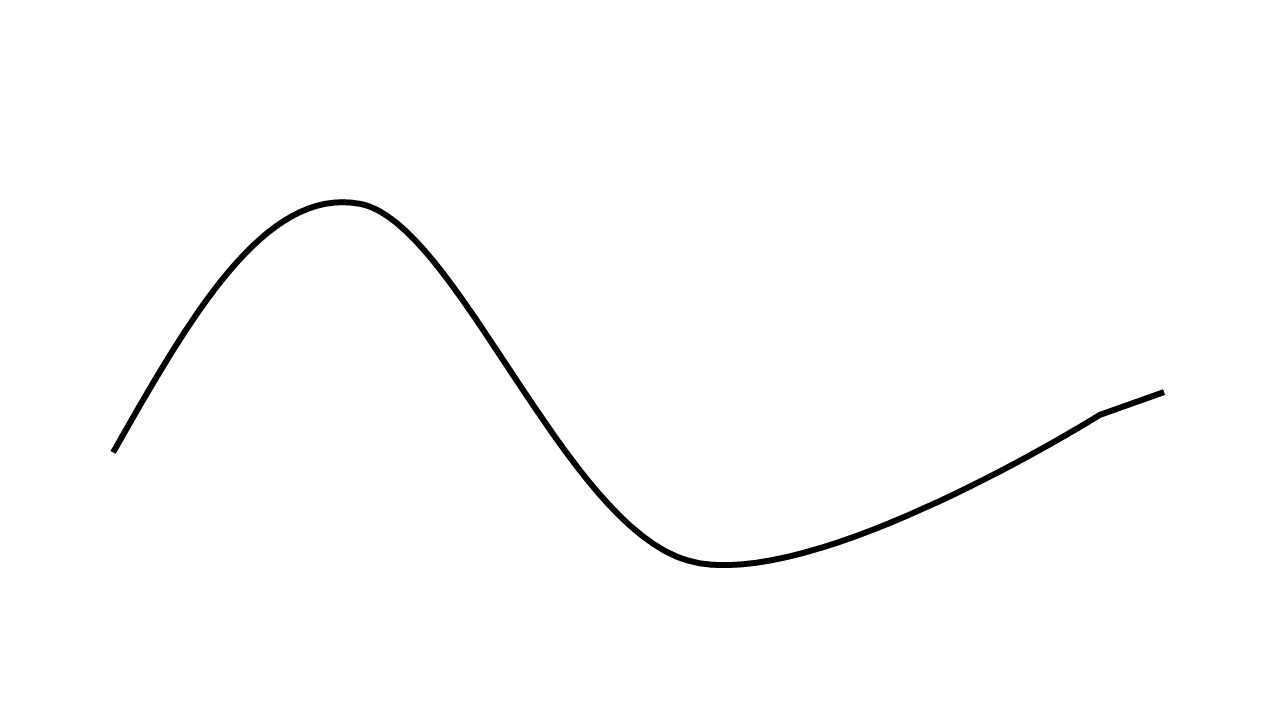
\includegraphics[width=5cm]{./figures/STover_1.png}
\caption{开弦.} \label{STover_fig1}
\end{figure}
\begin{figure}[ht]
\centering
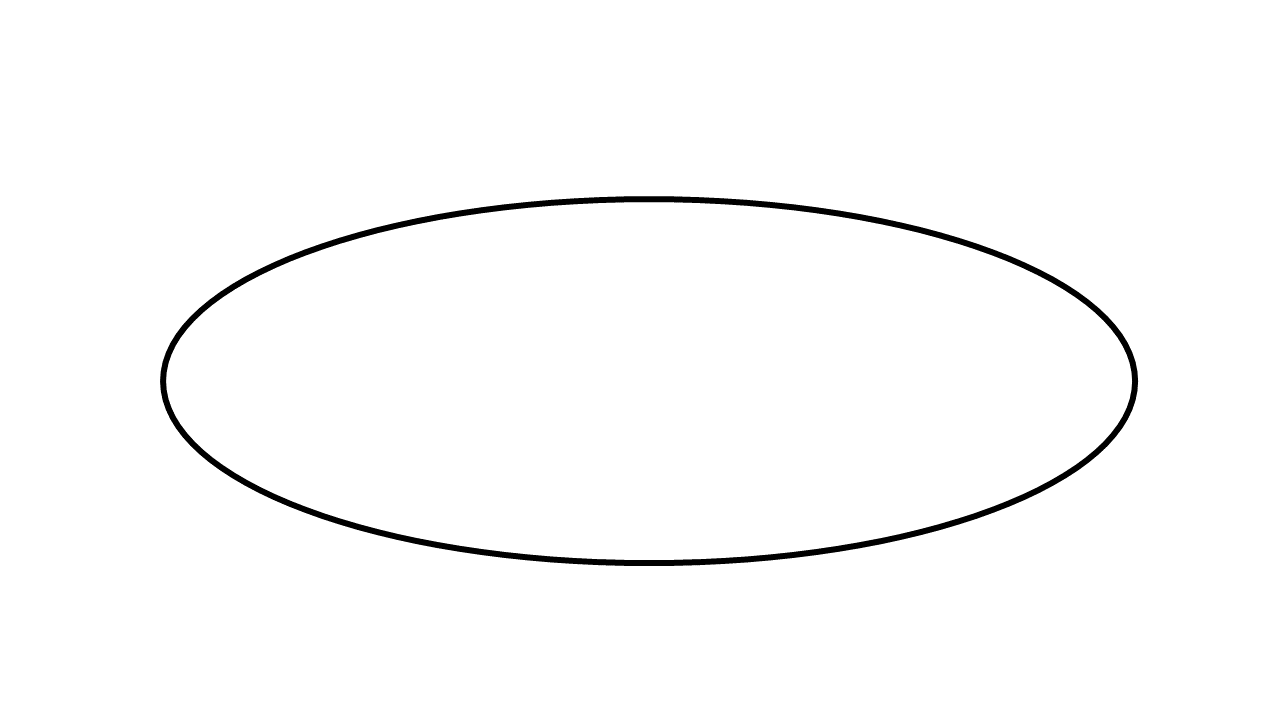
\includegraphics[width=5cm]{./figures/STover_2.png}
\caption{闭弦.} \label{STover_fig2}
\end{figure}
弦的激发给出了各种不同的粒子.粒子在时空中运动的轨迹叫做\textbf{世界线(world line)}.弦在时空中运动的轨迹叫做\textbf{世界面(world sheet)}.世界面由两个参数$\sigma$和$\tau$来参数化.函数$x^\mu(\tau,\sigma)$ 把世界面上的坐标$\sigma$和$\tau$映射到时空坐标$x$上.

\begin{figure}[ht]
\centering
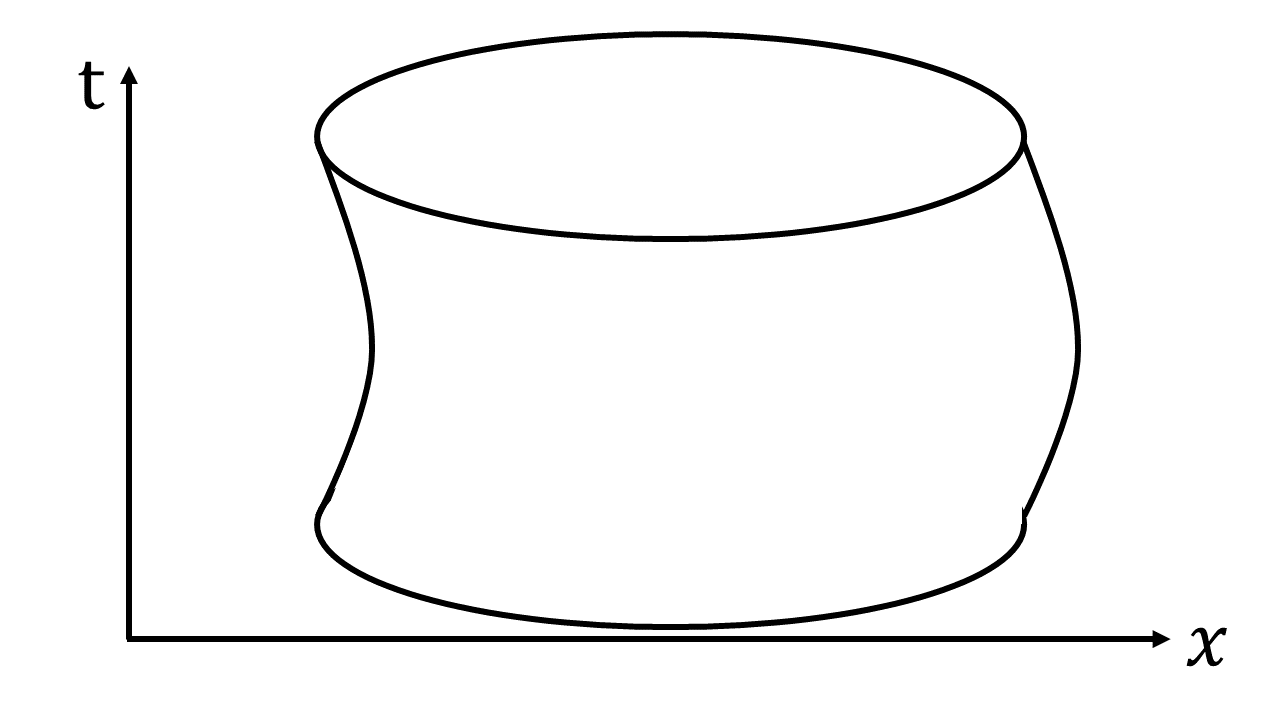
\includegraphics[width=5cm]{./figures/STover_3.png}
\caption{世界面$x^\mu (\tau,\sigma)$.} \label{STover_fig3}
\end{figure}

\begin{figure}[ht]
\centering
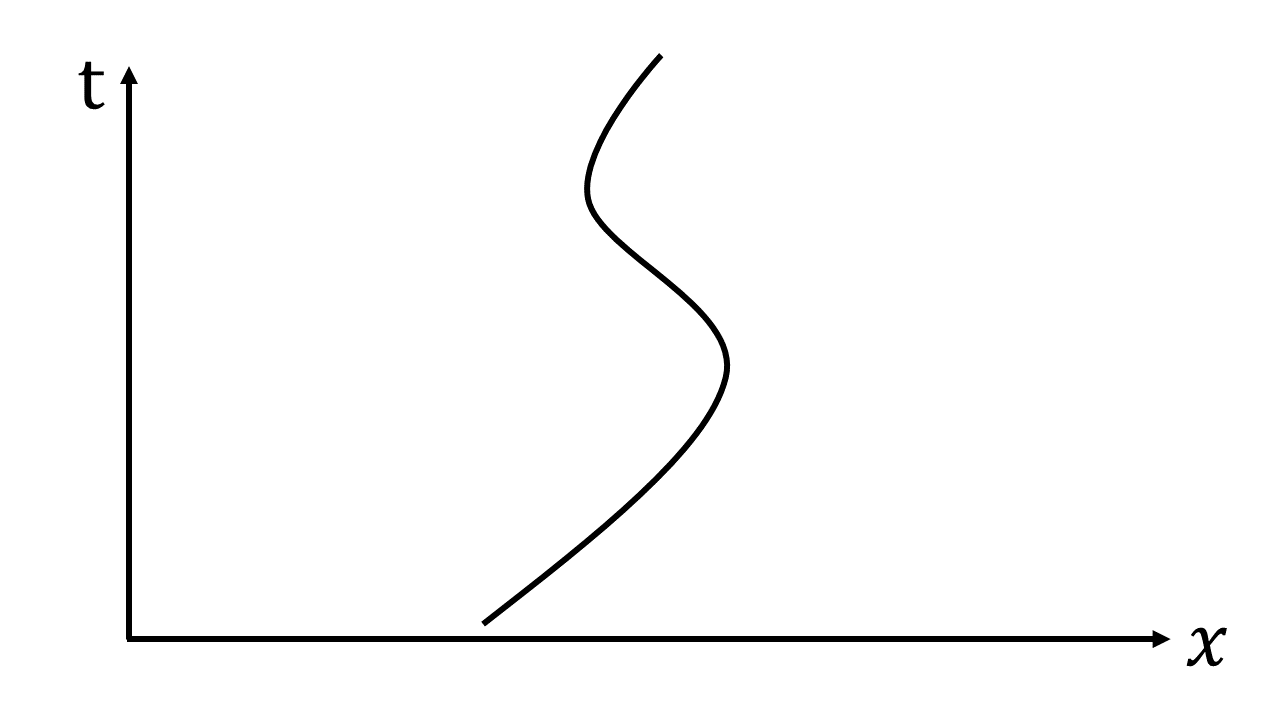
\includegraphics[width=5cm]{./figures/STover_4.png}
\caption{世界线$x^\mu(\tau)$.} \label{STover_fig4}
\end{figure}

在弦论世界里面,组成物质的基本单元是长度大约是普朗克长度($10^{-33}\Si{cm}$)的弦.像所有其他弦一样,这些基本弦能够振动.不同的振动频率形成了不同性质的粒子.对于一个自旋为$J$质量为$m_J$的粒子,质量和自旋通过如下式子联系起来
\begin{align}
J = \alpha' m_J^2~.
\end{align}

弦也能分开和合并.比如弦A可以分开变成弦B和弦C.这个过程对应于粒子衰变
\begin{align}
A \rightarrow B + C~.
\end{align}


